\documentclass[presentation]{beamer}
\usepackage[utf8]{inputenc}
\usepackage[T1]{fontenc}
\usepackage{fixltx2e}
\usepackage{graphicx}
\usepackage{longtable}
\usepackage{float}
\usepackage{wrapfig}
\usepackage{rotating}
\usepackage[normalem]{ulem}
\usepackage{amsmath}
\usepackage{textcomp}
\usepackage{marvosym}
\usepackage{wasysym}
\usepackage{amssymb}
\usepackage{hyperref}
\tolerance=1000
\usepackage{graphicx} \DeclareMathOperator{\argmin}{argmin}

\newcommand{\me}{\mathrm{e}}
\providecommand{\e}[1]{\ensuremath{\times 10^{#1}}} 
\providecommand{\mb}[1]{\mathbf{#1}}
\providecommand{\mf}[1]{\mathbf{#1}}
\providecommand{\ro}[1]{\mathbf{\mathbf{r}}_o}
\providecommand{\so}[1]{\mathbf{\hat{s}}_o}
\providecommand{\rb}[1]{\mathbf{r}_b}
\providecommand{\rbm}[1]{r_b^{\text{m}}}
\providecommand{\rd}[1]{\mathbf{r}_d}
\providecommand{\mh}[1]{\mathbf{\hat{#1}}}
\providecommand{\mbb}[1]{\mathbb{#1}}
\providecommand{\bs}[1]{\boldsymbol{#1}} 
\providecommand{\intinf}{\int_{-\infty}^{\infty}}



\newcommand{\under}[2]{\underset{\scriptscriptstyle#1}{#2}}


\usetheme{simple}
\usecolortheme{}
\usefonttheme{serif}
\useinnertheme{}
\useoutertheme{}
\author{Talon Chandler}
\date{May 23, 2018}
\title{Update on multiframe polarized light microscope singular spectra}

\begin{document}

\maketitle
\begin{frame}{Product of functions in harmonic coefficient space}
  \begin{align}
  f(\mh{p}) = \sum_{n=0}^\infty c_nz_n(\mh{p}), \qquad f'(\mh{p}) = \sum_{n'=0}^\infty c_{n'}'z_{n'}(\mh{p}). 
  \end{align}
The product of these two functions is
\begin{align}
  f''(\mh{p}) &= f(\mh{p})f'(\mh{p})=\sum_{n=0}^\infty \sum_{n'=0}^\infty c_n c_{n'}' z_n(\mh{p}) z_{n'}(\mh{p}) = \sum_{n''=0}^{\infty} c_{n''}''z_{n''}(\mh{p}), \label{eq:two}
  \end{align}
\end{frame}

\begin{frame}{Product of harmonics in coefficient space}
    \begin{align}
      c_{n''}'' &= \sum_{n=0}^\infty \sum_{n'=0}^\infty P_{n,n',n''} c_n c_{n'}',\quad \text{or}\\
      {c''}^{n''} &= P^{n''}_{n,n'} c^{n} {c'}^{n'}\quad \text{in Einstein notation.}
    \end{align}
    \begin{align}
    P_{n,n',n''} = \int_{\mbb{S}^1}d\mh{p}\, z_{n}(\mh{p})z_{n'}(\mh{p})z_{n''}(\mh{p}).\label{eq:triple}
    \end{align}
  \end{frame}

\begin{frame}{Product of circular and spherical harmonics}
\begin{align}
  {c''}^{n'', j''} = P_{n,n'}^{n''} G_{j,j'}^{j''} c^{n,j} {c'}^{n', j'}.\label{eq:final}
\end{align}
where
\begin{align}
  P_{n,n',n''} &= \int_{\mbb{S}^1}d\mh{p}\, z_{n}(\mh{p})z_{n'}(\mh{p})z_{n''}(\mh{p}).\label{eq:triple}\\
  G_{j,j',j''} &= \int_{\mbb{S}^2}d\mh{s}\, y_{j}(\mh{s})y_{j'}(\mh{s})y_{j''}(\mh{s}).
\end{align}.

In \texttt{numpy}:
\begin{align}
  \texttt{np.einsum(`abc,def,ad,be->cf', P, G, c1, c2)}
\end{align}
\end{frame}

% \begin{frame}{Continuous model $\mbb{L}_2(\mbb{R}^2 \times \mbb{S}^2) \rightarrow \mbb{L}_2(\mbb{R}^{2}\times \mbb{S}^1)$}
%   \vspace{-2em}
%   \begin{align*}
%     \intertext{Forward model:}
%     [\mathcal{H}f](\rd{}, \hat{\mb{p}}) = \int_{\mbb{S}^2}d\so{}\int_{\mbb{R}^2}d\ro{}\, h(\rd{} -\ro{}, \so{}; \hat{\mb{p}})f(\ro{}, \so{}),
%   \end{align*}
%     \begin{align*}    
%     \intertext{Adjoint:}
%     [\mathcal{H}^{\dagger}g](\ro{}, \so{}) = \int_{\mbb{S}^1}d\hat{\mb{p}}\, \int_{\mbb{R}^2}d\mb{r}_{d}\, h(\rd{} - \ro{}, \so{}; \hat{\mb{p}})g(\rd{}, \hat{\mb{p}}).
%     \end{align*}
%   \end{frame}

\begin{frame}[label=sec-1]{Single-view polarized illumination transfer function}
      \centering
      \includegraphics[width=1.0\columnwidth]{figs/Hill.pdf}
    \end{frame}

\begin{frame}[label=sec-1]{Single-view polarized detection transfer function}
      \centering
      \includegraphics[width=1.0\columnwidth]{figs/Hdet.pdf}
\end{frame}

\begin{frame}[label=sec-1]{Single-view polarized illumination singular spectrum}
      \centering
      \includegraphics[width=1.0\columnwidth]{figs/SVSill.pdf}
    \end{frame}

\begin{frame}[label=sec-1]{Single-view polarized detection singular spectrum}
      \centering
      \includegraphics[width=1.0\columnwidth]{figs/SVSdet.pdf}
\end{frame}

\begin{frame}[label=sec-1]{Symmetry group for both polarized illumination and detection}
      \centering
      \includegraphics[width=1.0\columnwidth]{figs/symmetry.pdf}
\end{frame}


% \begin{frame}{Polarized illumination SVD}
% \begin{align*}
%   \mu_{\bs{\rho},0} &= \{H_{0,0}^{0}(\rho)\}^2 + \{H_{2,0}^{0}(\rho)\}^2 + \{H_{4,0}^{0}(\rho)\}^2,\\
%   \mu_{\bs{\rho},1} = \mu_{\bs{\rho},2} &= \{H_{2,2}^{2}(\rho)\}^2 + \{H_{4,2}^{2}(\rho)\}^2,
% \end{align*}
% \begin{align*}
%   u_{\bs{\rho},0}(\ro{}, \so{}) &= \me{}^{i2\pi\bs{\rho}\cdot\ro{}}[H_{0,0}^0(\rho)y_0^0(\so{}) + H_{2,0}^0(\rho)y_2^0(\so{}) + H_{4,0}^0(\rho)y_4^0(\so{})],\\
%   u_{\bs{\rho},1}(\ro{}, \so{}) &= \me{}^{i2\pi\bs{\rho}\cdot\ro{} }[H_{2,-2}^{-2}(\rho)y_2^{-2}(\so{}) + H_{4,-2}^{-2}(\rho)y_4^{-2}(\so{})],\\
%   u_{\bs{\rho},2}(\ro{}, \so{}) &= \me{}^{i2\pi\bs{\rho}\cdot\ro{} }[H_{2,2}^2(\rho)y_2^2(\so{}) + H_{4,2}^2(\rho)y_4^2(\so{})].
%     \end{align*}
% \begin{align*}
%   v_{\bs{\rho},0}(\rd{}, \mh{p}) &= \me{}^{i2\pi\bs{\rho}\cdot\rd{}}z_0(\mh{p}),\\
%   v_{\bs{\rho},1}(\rd{}, \mh{p}) &= \me{}^{i2\pi\bs{\rho}\cdot\rd{}}z_{-2}(\mh{p}),\\
%   v_{\bs{\rho},2}(\rd{}, \mh{p}) &= \me{}^{i2\pi\bs{\rho}\cdot\rd{}}z_2(\mh{p}).
% \end{align*}
% \end{frame}

% \begin{frame}[label=sec-1]{Symmetries}
%       \centering
%       \includegraphics[width=1.0\columnwidth]{symmetry.pdf}
% \end{frame}




  
\end{document}